\section{Empirical Methodology}
\label{sec:empirical}
%To evaluate HIGHLIGHTS and HIGHLIGHTS-DIV, we conducted experiments in which participants were shown summaries produced by these algorithms, as well as summaries produced by baseline methods. We next describe the empirical domain used in our experiment, the experimental conditions and the 
\paragraph{Empirical Domain.} To evaluate HIGHLIGHTS and HIGHLIGHTS-DIV, We generated summaries of agents playing the Mrs. Pacman game~\cite{rohlfshagen2011ms}. Figure~\ref{fig:pacman} shows a screen from the experiment which includes snapshots of the Pacman maze used in our experiments. This game configuration includes two types of food pellets: regular pellets (small dots) are worth 10 points each and power pellets (larger dots) are worth 50 points each. After eating a power pellet, ghosts become edible for a limited time period. Pac-Man receives 200 points for each ghost it eats. Ghosts chase Pac-Man with $80\%$ probability and otherwise move randomly. In each state, Pac-Man has at most four moves (right, left, up or down). Important states in the game include situations where Pacman is very close to ghosts (e.g., the state shown for the Pacman game on the right side in Figure~\ref{fig:pacman}) or  when Pacman has an opportunity to eat a power pellet, or a ghost. 

Due to the large size of the state space, we used the high-level 7-feature representation from Torrey \& Taylor's~\shortcite{torrey2013teaching} implementation. Q-values are defined as a weighted function of the feature values, i.e., $Q(s,a)=\omega_{0}+\sum_{i}{\omega_{i} \cdot f_{i}(s,a)}$
% \begin{equation}
% Q(s,a)=\omega_{0}+\sum_{i}{\omega_{i} \cdot f_{i}(s,a)}
% \label{e:q}
% \vspace{-0.3cm}
% \end{equation}  


\begin{figure}[h]
	\centering
    \frame{
	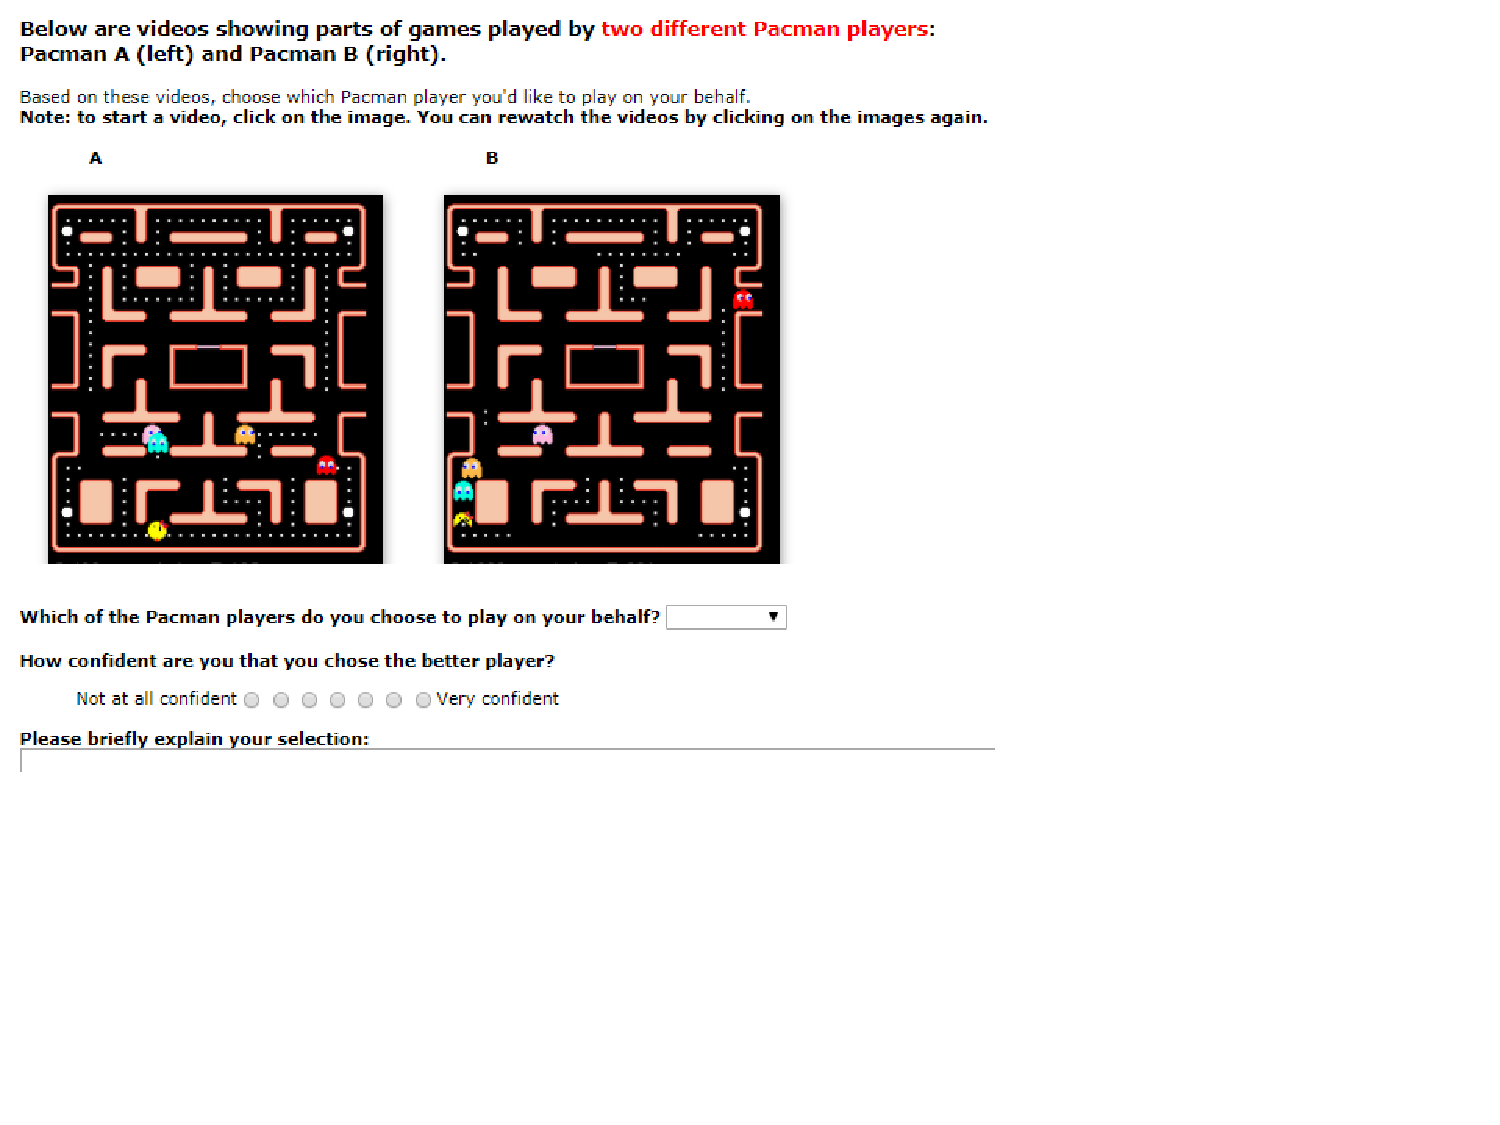
\includegraphics[width=0.98\columnwidth]{figs/pacman.pdf}}\\
	\caption{A screenshot of the agent selection task.}
	\label{fig:pacman}
	\vspace{-0.4cm}
\end{figure}


% \begin{figure}
% 	\centering
% 	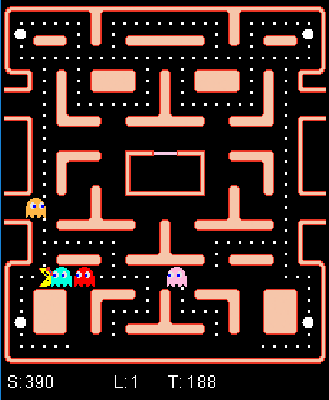
\includegraphics[width=0.3\columnwidth]{figs/pacman1.pdf}\\
% 	\caption{The Mrs. Pac-Man Game.}
% 	\label{fig:pacman}
% 	\vspace{-0.4cm}
% \end{figure}




\paragraph{Experimental Conditions.} In addition to generating summaries using the two versions of the HIGHLIGHTS algorithm, we also generated summaries using two baseline methods:
\begin{itemize}[leftmargin=.3cm]
\item \emph{First}: a summary is generated from the first $k$ trajectories Pacman encounters. This baseline is akin to having a user watch the agent act (e.g., watching a video of an autonomous vehicles driving) until she runs out of time.
\item \emph{Random}: a summary is generated by sampling $k$ trajectories uniformly from the agent's execution trace. %Since we generate the summaries online, we used reservoir sampling~\cite{vitter1985random} which extracts random samples from an online stream. 
With this baseline states that are more frequently encountered are more likely to be selected to the summary. 
\end{itemize}

The parameter values for the algorithms used to generate the Pacman summaries are listed in Table~\ref{tb:parameters}.  All summaries included five trajectories ($k=5$), each showing 40 neighboring states ($l$=40). 
%We used $statesAfter=10$, meaning that each trajectory included 10 states following the important state (the first 29 states were the states preceding the important state). 
They enforced a gap of 50 states before considering a state for inclusion in the summary (i.e., $intervalSize = 50$).  To present the summaries to users, we generated video-clips (GIF files) showing the trajectories that were chosen for the summary\footnote{See example summary video here: \url{https://goo.gl/79dqsd}.}. We note that the summaries shown to participants did not include the current score of the agent (see Figure~\ref{fig:pacman}) to ensure that participants' evaluation will  be based on the observed behavior of the Pacman player rather than its score.

We generated three different agents by varying their training period. The lowest performing agent was trained for 200 episodes (scores 2262 points on average), the medium agent for 400 episodes (scores 2732 points on average), and the highest performing agent was trained for 2000 episodes (scores 3826 points on average). Henceforth, we refer to these agents as the \emph{200E}, \emph{400E} and \emph{2000E} agent, respectively. Generating agents of varying performance enabled us to have a ground truth when asking participants to assess the agents' performance. The summaries were generated after the agents were fully trained and reflect the final policies of the agents.  



%Participants completed two types of task, described in more detail in Section~\ref{sec:procedure}. In the first task, participants were shown summaries of two different agents, and were asked to choose which agent they want to play on their behalf. This task provides an objective way of assessing whether the summaries helped participants assess the performance of different agents. In the second task, participants were shown two summaries of \emph{the same} agent, and were asked which summary they found more helpful for assessing the agent's capabilities. This task provided a subjective measure assessing the perceived usefulness of the summaries. For these tasks, we generated three different agents by varying their training period. The lowest performing agent was trained for 200 episodes, the medium agent for 400 episodes, and the highest performing agent was trained fro 2000 episodes. Henceforth we refer to these agents as the \emph{200E}, \emph{400E} and \emph{2000E} agent, respectively. Generating agents of varying performance enabled us to have a ground truth for the agent selection task. The summaries were generated after the agents were fully trained, such that they reflect the final policies of the agents.  

We conducted two experiments. Experiment 1 compared the HIGHLIGHTS algorithm with the two baseline methods. Experiment 2 compared the HIGHLIGHTS-DIV algorithm with the basic HIGHLIGHTS algorithm and the \emph{Random} baseline. We used the same procedure in both experiments. 

\paragraph{Procedure}
%\label{sec:procedure}
Participants were first shown a tutorial explaining the rules of the Pacman game. They then had to pass a quiz ensuring they read and understood the rules. Next, they were asked to complete two different tasks (described next). Participants received a base payment of \$1.5, and could earn a bonus of up to \$0.9 (explained in task 1). We used a within-subject study design, such that all participants evaluated all summary methods. 
%An anonymized version of the study (without the consent form) can be accessed here ***add url***. 

\textbf{Task 1: Agent Selection.}
In the first task, participants were shown pairs of  summaries of two \emph{different} Pacman agents, produced by the \emph{same} summary method (e.g., a HIGHLIGHTS summary of the \emph{200E} agent and a HIGHLIGHTS summary of the \emph{400E}). They were asked to choose the agent they would like to play on their behalf. Participants were also asked to explain their selection and to rate their confidence in their decision on a 7-point Likert scale (1 - not at all confident to 7 - very confident). Overall, there were 9 such pairs (3 agent levels X 3 summarization methods).  An example agent selection task is shown in Figure~\ref{fig:pacman}. The ordering of pairs to compare as well as which summary was shown on the left and which on the right were randomized. Participants were given a bonus of 10 cents for each correct agent selection, such that they had a monetary incentive to select the better performing agent. 

The different agent comparisons differed in the difficulty of identifying the better agent: the \emph{200E} and \emph{400E} agents had the most similar performance, resulting in a \emph{high-difficulty} comparison; the \emph{200E} and \emph{2000E} agents differed most substantially in their performance, resulting in a \emph{low-difficulty} comparison; we refer to the comparison of  the \emph{400E} and \emph{2000E} agents as the \emph{medium-difficulty} comparison, as the differences in the agents' policies were more substantial than for the \emph{200E} and \emph{400E} agents, but less substantial than for the \emph{200E} and \emph{2000E} agents. 

\textbf{Task 2: Summary Preferences.}
While the first task measured participants' objective ability to identify the better agent, in the second task we elicited participants' subjective opinions about the helpfulness of different summaries. They were again shown pairs of summaries. This time the two summaries were of \emph{the same} agent (participants were told it was the same agent), but were generated by a \emph{different} summary method (e.g., comparing a HIGHLIGHTS summary of the 200E agent with a \emph{Random} summary of the 200E agent). Participants were asked to rate which of the summaries they find more helpful for assessing the capabilities of the Pacman agent using a 7-point Likert scale (1 - video A is more helpful, 7 - video B is more helpful). They were also asked to provide a short explanation for their preference. 

To maintain a reasonable experiment length and because we were primarily interested in the usefulness of HIGHLIGHTS summaries, in this task participants only made 4 comparisons (2 of the 3 agents, comparing HIGHLIGHTS summaries with each of the baseline summaries). The ordering of pairs to compare as well as their location on the screen (left or right) were randomized. 

\paragraph{Evaluation Metrics and Analyses}
The analysis of task 1 evaluated participants' correctness rate when selecting Pacman agents with each summary method. We analyzed the data using a logistic regression, controlling for the comparison type (200E vs. 400E agents, 400E vs. 2000E agents or 200E vs. 2000E agents). Since we used a within-subject design, we ran a repeated measures logistic regression. We also compared participants' confidence in making these selections. Confidence ratings were analyzed using an ordinal logistic regression, again controlling for the comparison type.  For the fitted regression models, we report the significance of the coefficients as well as the odds ratio values ($OR$), which can be interpreted as effect sizes. Values between 1.5 and 3 are interpreted as a small effect, between 3 and 5 as medium, and above 5 as large~\cite{borenstein2009converting,chen2010big}.

When analyzing task 2, we compared the helpfulness ratings given to the summaries. We normalized the preferences such that 7 always means ``HIGHLIGHTS is more helpful'' and 1 means ``[other method] is more helpful''. That is, a rating greater than 4 indicates a preference for HIGHLIGHTS. We analyzed these ratings using the non-parametric Wilcoxon rank sum test.\footnote{We used Wilcoxon rank sum as the scale was ordinal and the data was not normally distributed. However, we obtain similar results when using standard t-test.}

To account for multiple hypotheses testing, we adjusted p-values with the Holm's sequentially rejective Bonferroni procedure~\cite{holm79:simple,shaffer95:multiple}. We report raw p-values, but in all cases we state significant differences, the adjusted p-values were also smaller than $0.05$.




